\section{An Introduction to the Greek Alphabet}
\AUTHOR{Jonathan Webley} \\
The first pure alphabet emerged around 2000 BCE in Egypt, based on alphabetic principles of the Egyptian hieroglyphs and is called the Proto-Sinaitic alphabet. Surprisingly, nearly every alphabet in the world today either descends directly from it or was inspired by it.

Essentially, writing was independently invented only a handful of times. Virtually every symbol we see today in the West had as its ultimate origins the work of, probably, a single person, living in, probably, ancient Egypt. That idea was then copied and evolved and developed to become the tens of thousands of symbols, for example, found in Unicode.

An important descendant of the Proto-Sinaitic alphabet was the Phoenician alphabet, which in turn evolved into the Arabic, Hebrew and Greek alphabets. Indian scripts such as Devanagari are also descendants of the Phoenician alphabet. All the modern scripts of Europe -- such as Latin, Gothic and Cyrillic -- are descended from the Greek alphabet. Our word \emph{alphabet} derives from the Greek letters \emph{alpha} and \emph{beta}.

% -------------------------------
\subsection{Math mode}
Because of its widespread use in mathematics, science and engineering the Greek alphabet is a standard feature of \TeX\ when in math mode. There are codes for every lowercase letter with the exception of omicron, because it has the same shape as the Latin ``\texttt{o}''. The math mode versions of the lowercase Greek letters are in italics whereas the uppercase letters are upright.

% -------------------------------
\begin{figure}[h]
	\centering
		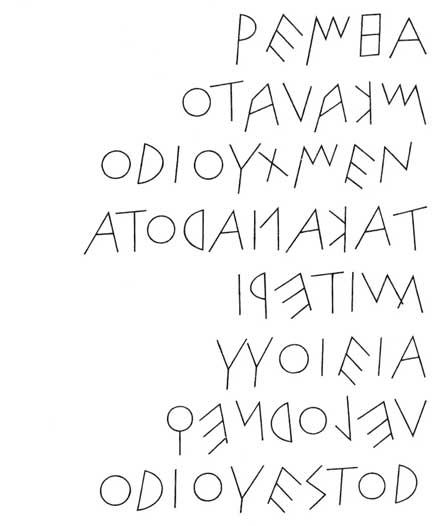
\includegraphics[width=0.85\textwidth]
		            {Greek_Inscription.jpg}
	\caption*{Greek Inscription, 5th century BCE}
	\label{fig:Greek_Inscription}
\end{figure}

% -------------------------------
\subsection{Babel}
Using the \texttt{greek} option of the \texttt{babel} package is the normal way to write text in Greek. If the whole document is in Greek then the preamble would include: \\
\indent $\backslash$\texttt{usepackage[greek]\{babel\}} \\
Each Latin letter in the \texttt{tex} file is then automatically transliterated to its equivalent Greek letter. These equivalences are given in the tables below.

A document such as this one, containing mainly English with a smattering of Greek, would have: \\
\indent $\backslash$\texttt{usepackage[greek,english]\{babel\}} \\
and in the body when Greek is required: \\
\indent $\backslash$\texttt{foreignlanguage\{greek\}\{Alpha\}} \\
which renders as \foreignlanguage{greek}{Alpha}.
\LaTeX\ also has other ways of achieving this result which are not detailed here.

The \texttt{greek} option of this package also includes three obsolete letters as illustrated below. The \LaTeX\ codes for these letters are: $\backslash$\texttt{qoppa}, $\backslash$\texttt{sampi} and $\backslash$\texttt{stigma} and these are shown later.

% -------------------------------
\subsection{The Letters}
 There are 24 letters in the modern Greek alphabet, with uppercase and lowercase variants. These letters are given in the following tables, and the columns in it are:
\begin{enumerate}
	\item Greek letter produced in math mode by standard \TeX.
	\item The \TeX\ code for this letter (the letter name).
	\item Greek letter produced by the \texttt{babel} package.
	\item The Latin letter used to produce this letter.
\end{enumerate}

\smallskip
\begin{table}[H]
	\centering
	\caption* {Lowercase letters}
		\begin{tabular}{cp{3.2cm}cc}
		  \toprule
			\LaTeX\    & \LaTeX\   & Latin  & Latin \\
			letter          & code         & letter &       \\ 
\midrule
$\alpha$                  & \texttt{$\backslash$alpha}  & \foreignlanguage{greek}{a} & a \\
$\beta$                   & \texttt{$\backslash$beta}   & \foreignlanguage{greek}{b} & b \\
$\gamma$                  & \texttt{$\backslash$gamma}  & \foreignlanguage{greek}{g} & g \\
$\delta$                  & \texttt{$\backslash$delta}  & \foreignlanguage{greek}{d} & d \\
$\epsilon$, $\varepsilon$ & \texttt{$\backslash$epsilon},  \texttt{$\backslash$varepsilon} & \foreignlanguage{greek}{e} & e \\
$\zeta$                   & \texttt{$\backslash$zeta}   & \foreignlanguage{greek}{z} & z \\
$\eta$                    & \texttt{$\backslash$eta}    & \foreignlanguage{greek}{h} & h\\
$\theta$, $\vartheta$     & \texttt{$\backslash$theta}, \texttt{$\backslash$vartheta} & \foreignlanguage{greek}{j} & j \\
$\iota$                   & \texttt{$\backslash$iota}   & \foreignlanguage{greek}{i} & i \\
$\kappa$                  & \texttt{$\backslash$kappa}  & \foreignlanguage{greek}{k} & k \\
$\lambda$                 & \texttt{$\backslash$lambda} & \foreignlanguage{greek}{l} & l \\
$\mu$                     & \texttt{$\backslash$mu}     & \foreignlanguage{greek}{m} & m \\
$\nu$                     & \texttt{$\backslash$nu}     & \foreignlanguage{greek}{n} & n \\
$\xi$                     & \texttt{$\backslash$xi}     & \foreignlanguage{greek}{x} & x \\
$o$                       & o (omicron)                 & \foreignlanguage{greek}{o} & o \\
$\pi$, $\varpi$           & \texttt{$\backslash$pi}, \texttt{$\backslash$varpi}      &  \foreignlanguage{greek}{p} & p \\
$\rho$, $\varrho$         & \texttt{$\backslash$rho}, \texttt{$\backslash$varrho}    & \foreignlanguage{greek}{r}  & r \\
$\sigma$, $\varsigma$     & \texttt{$\backslash$sigma}, \texttt{$\backslash$varsigma} & \foreignlanguage{greek}{s} & s \\
$\tau$                    & \texttt{$\backslash$tau}                                  & \foreignlanguage{greek}{t} & t \\
$\upsilon$                & \texttt{$\backslash$upsilon}                              & \foreignlanguage{greek}{u} & u \\
$\phi$, $\varphi$         & \texttt{$\backslash$phi}, \texttt{$\backslash$varphi}     & \foreignlanguage{greek}{f} & f \\
$\chi$                    & \texttt{$\backslash$chi}                                  & \foreignlanguage{greek}{q} & q \\
$\psi$                    & \texttt{$\backslash$psi}                                  & \foreignlanguage{greek}{y} & y \\
$\omega$                  & \texttt{$\backslash$omega}                                & \foreignlanguage{greek}{w} & w \\
\bottomrule
		\end{tabular}
\end{table}

\smallskip

Many of the uppercase letters are simply those used in the Latin alphabet, and for these there is no \TeX\ code. 
% In this case, the letter name is given in brackets.

%\medskip
\begin{table}[H]
\centering
\caption* {Uppercase letters}
\begin{tabular}{cp{2.5cm}cc}
\toprule
\LaTeX\    & \LaTeX\   & Latin  & Latin \\
letter     & code      & letter &       \\ 
\midrule
A            & A (alpha)                    & \foreignlanguage{greek}{A} & A \\
B            & B (beta)                     & \foreignlanguage{greek}{B} & B \\
\bottomrule
\end{tabular}
\end{table}


\begin{table}[H]
\centering
\caption* {Uppercase letters (cont.)}
\begin{tabular}{cp{3.2cm}cc}
\toprule
\LaTeX\    & \LaTeX\   & Latin  & Latin \\
letter     & code      & letter &       \\ 
\midrule
$\Gamma$     & \texttt{$\backslash$Gamma}   & \foreignlanguage{greek}{G} & G \\
$\Delta$     & \texttt{$\backslash$Delta}   & \foreignlanguage{greek}{D} & D \\
E            & E (epsilon)                  & \foreignlanguage{greek}{E} & E \\
Z            & Z (zeta)                     & \foreignlanguage{greek}{Z} & Z \\
H            & H (eta)                      & \foreignlanguage{greek}{H} & H \\
$\Theta$     & \texttt{$\backslash$Theta}   & \foreignlanguage{greek}{J} & J \\
I            & I (iota)                     & \foreignlanguage{greek}{I} & I \\
K            & K (kappa)                    & \foreignlanguage{greek}{K} & K \\
$\Lambda$    & \texttt{$\backslash$Lambda}  & \foreignlanguage{greek}{L} & L \\
M            & M (mu)                       & \foreignlanguage{greek}{M} & M \\
N            & N (nu)                       & \foreignlanguage{greek}{N} & N \\
$\Xi$        & \texttt{$\backslash$Xi}      & \foreignlanguage{greek}{X} & X \\
O            & O (omicron)                  & \foreignlanguage{greek}{O} & O \\
$\Pi$        & \texttt{$\backslash$Pi}      & \foreignlanguage{greek}{P} & P \\
P            & P (rho)                      & \foreignlanguage{greek}{R} & R \\
$\Sigma$     & \texttt{$\backslash$Sigma}   & \foreignlanguage{greek}{S} & S \\
T            & T (tau)                      & \foreignlanguage{greek}{T} & T \\
$\Upsilon$   & \texttt{$\backslash$Upsilon} & \foreignlanguage{greek}{U} & U \\
$\Phi$       & \texttt{$\backslash$Phi}     & \foreignlanguage{greek}{F} & F \\
X            & X (chi)                      & \foreignlanguage{greek}{Q} & Q \\
$\Psi$       & \texttt{$\backslash$Psi}     & \foreignlanguage{greek}{Y} & Y \\
$\Omega$     & \texttt{$\backslash$Omega}   & \foreignlanguage{greek}{W} & W \\
\bottomrule
\end{tabular}
\end{table}

\smallskip

Upright versions of the Greek letters can be found in \texttt{pxfonts}, \texttt{txfonts} and \texttt{upgreek}. 
There is also a variant of kappa found in the \texttt{amssymb} package: $\varkappa$ (\texttt{\$$\backslash$varkappa}\$).
The International Phonetic Alphabet uses various symbols, many of which are Greek letters or are derived from Greek letters. These can be found in various packages, including \texttt{phonetic}, \texttt{wsuipa} and \texttt{t4phonet}.

% -------------------------------
\subsection{Bold Greek}
The simplest way to produce bold Greek text is with the \texttt{babel} package: \\
\indent \texttt{$\backslash$textbf\{$\backslash$foreignlanguage\{greek\}\{Lambda\}\}} \\
which produces: \\
\indent \textbf{\foreignlanguage{greek}{Lambda}}

In math mode things are more complicated: \texttt{textbf} is not valid; \texttt{mathbf} only makes bold the uppercase letters. In package \texttt{amsbsy} the command \texttt{boldsdymbol} will make all symbols bold. Command \texttt{pmb} produces heavy symbols which  resembles bold. The \texttt{bm} package has a command \texttt{bm} which makes all maths bold. And finally, package \texttt{fixmath} has a command \texttt{mathbold} which can also be used.


% -------------------------------
\subsection{Obsolete letters}
There are a number of obsolete letters. The samples in the following table derive either from \texttt{amssymb} or from the \texttt{greek} option of the \texttt{babel} package.

The \texttt{arevmath} package is intended for presentations and posters and its use is not illustrated here. There are large and small forms of each letter, which otherwise seem identical.

%\bigskip
\begin{center}
\begin{tabular}{lcp{3.5cm}}
\toprule
Name & Letter & Packages \\
\midrule
digamma & $\digamma$                       & \texttt{amssymb}, \texttt{arevmath}  \\
het     &                                  & none known \\
koppa   &                                  & \texttt{arevmath}           \\
qoppa   & \foreignlanguage{greek}{\qoppa}  & \texttt{arevmath}, \texttt{babel}    \\
sampi   & \foreignlanguage{greek}{\sampi}  & \texttt{arevmath}, \texttt{babel}    \\
san     &                                  & none known \\
sho     &                                  & none known \\
stigma  & \foreignlanguage{greek}{\stigma} & \texttt{arevmath}, \texttt{babel}    \\
\bottomrule
\end{tabular}
\end{center}
%\bigskip

Qoppa and koppa refer to the same letter: its shape evolved from that referred to as qoppa to that referred to as koppa.

All of these letters are available in Unicode.

% -------------------------------
\subsection{Greek Diacritics}
Modern Greek uses only two diacritics, however, before 1982 Greek orthography was more complex. Modern Greek is called monotonic (meaning ``single accented''), while the older orthography is called polytonic (meaning ``many accented''). The \texttt{babel} package by default uses the modern orthography, but the following preamble allows the older orthography to be used: \\
\indent $\backslash$\texttt{usepackage[greek]\{babel\}} \\
\indent $\backslash$\texttt{languageattribute\{greek\}\{polutoniko\}} \\
The latter option, ``polutoniko'', is the Greek for ``polytonic''.

Use of this option is not illustrated here.

% -------------------------------
\subsection{Some uses}
A couple of letters can be found in the \texttt{textcomp} and \texttt{gensymb} packages:

%\smallskip

\begin{center}
\begin{tabular}{ccc}
\toprule
Symbol   & \texttt{textcomp} & \texttt{gensymb} \\
\midrule
\textohm & $\backslash$\texttt{textohm} & $\backslash$\texttt{ohm} \\
\textmu  & $\backslash$\texttt{textmu}  & $\backslash$\texttt{micro} \\
\bottomrule
\end{tabular}
\end{center}

%\smallskip

This version of \textit{mu} is used for the SI prefix micro- for $10^{-6}$. For example, the symbol for a micron is \texttt{\textmu m}.

Mathematics uses variants of \textit{sigma} and \textit{pi} as operators, such that in display mode subscripts and superscripts are placed beneath or above the letters respectively. These symbols are found in the \texttt{amssymb} package:

\smallskip

\begin{tabular}{cc}
$\displaystyle \sum_{i=0}^{n}$  & \texttt{\$$\backslash$sum\_\{i=0\}\^{}n\$} \\
$\displaystyle \prod_{i=0}^{n}$ & \texttt{\$$\backslash$prod\_\{i=0\}\^{}n\$}
\end{tabular}

\medskip

A couple of symbols are inverted, and are found in the \texttt{amssymb} package:

\begin{tabular}{clp{4.2cm}}
$\mho$   & \texttt{$\backslash$mho}   & This is ohm spelt backwards, and is an unofficial symbol for the siemens. \\
$\nabla$ & \texttt{$\backslash$nabla} & This symbol is the \textit{del} operator in mathematics.
\end{tabular}


% -------------------------------
\subsection{Greek Arithmetic}
In Greek, there are no separate symbols, glyphs, for numbers. Modern Greek uses the same arabic numerals that we use. So, like the Romans, the ancient Greeks used letters to stand for numbers (unlike the arabic system where the symbols stand for digits). 

The earliest system used was the Attic system, which is similar to the system used by the Romans:

\medskip

\begin{center}
\begin{tabular}{rcc}
\toprule
 Arabic & Greek & Roman \\
\midrule
 1     & I         & I \\
 5     & $\Pi$     & V \\
10     & $\Delta$  & X \\
100    & H         & C \\
1,000  & X         & M \\
10,000 & M         &   \\
\bottomrule
\end{tabular}
\end{center}

\medskip

The letters used by the Greeks are the initial letters of the words for the numbers. Each letter represents a number, and the values are added (though the Romans also subtracted):
\[
4 = \text{IIII (Greek)} = \text{IV (Roman)}
\]
%\[
%6 = \Pi\text{I (Greek)} = \text{VI (Roman)}
%\]

A later system was the Ionian or Athenian system, which uses 27 letters (the modern 24 letters plus 3 obsolete letters):

%\smallskip

\begin{center}
\begin{tabular}{lrclrclr}
$\alpha$   & 1  && $\iota$    & 10 && $\rho$     & 100 \\
$\beta$    & 2  && $\kappa$   & 20 && $\sigma$   & 200 \\
$\gamma$   & 3  && $\lambda$  & 30 && $\tau$     & 300 \\
$\delta$   & 4  && $\mu$      & 40 && $\upsilon$ & 400 \\
$\epsilon$ & 5  && $\nu$      & 50 && $\phi$     & 500 \\
$\digamma$ & 6  && $\xi$      & 60 && $\chi$     & 600 \\
$\zeta$    & 7  && o          & 70 && $\psi$     & 700 \\
$\eta$     & 8  && $\pi$      & 80 && $\omega$   & 800 \\
$\theta$   & 9  && \foreignlanguage{greek}{\qoppa} & 90 && \foreignlanguage{greek}{\sampi} & 900 \\
\end{tabular}
\end{center}

This system is also additive. So, $123 = \rho\kappa\alpha$. Extensions to this system allow for larger numbers.

Package \texttt{$\backslash$athnum} can be used to convert numbers in arabic format to numbers in Ionian format.

% \medskip
